\documentclass[tikz, border=5pt]{standalone}
\usepackage{amsmath}
\usetikzlibrary{patterns}

\newcommand{\drawgrid}{
    \draw[step=1cm,gray,very thin] (0,0) grid (4,4);
}

\newcommand{\goalstates}[1]{
    \foreach\i in {#1} {
        \pgfmathsetmacro{\x}{mod (\i, 4)}
        \pgfmathsetmacro{\y}{int (\i / 4)}
        \fill[gray!20] (\x, 3-\y) rectangle (\x+1, 4-\y);
        \fill[pattern=north east lines, pattern color=gray!50] (\x, 3-\y) rectangle (\x+1, 4-\y);
    }
}

\begin{document}
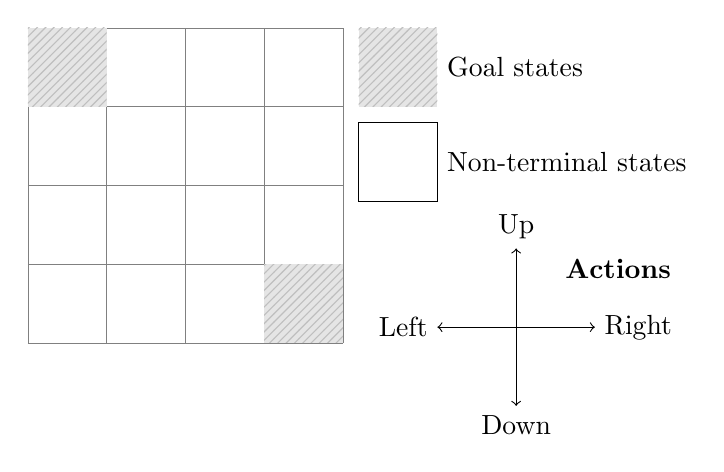
\begin{tikzpicture}
    % Grid and goal states
    \drawgrid
    \goalstates{0, 15}

    % Legend
    \fill[gray!20] (4.2,3) rectangle ++(1,1);
    \fill[pattern=north east lines, pattern color=gray!50] (4.2,3) rectangle ++(1,1);
    \node[right] at (5.2,3.5) {Goal states};
    \draw (4.2,1.8) rectangle ++(1,1);
    \node[right] at (5.2,2.3) {Non-terminal states};

    % Actions
    \coordinate (center) at (6.2,0.2);
    \draw[->] (center) -- ++(0,1) node[above] {Up};
    \draw[->] (center) -- ++(0,-1) node[below] {Down};
    \draw[->] (center) -- ++(-1,0) node[left] {Left};
    \draw[->] (center) -- ++(1,0) node[right] {Right};
    \node[above right=0.5cm] at (center) {\textbf{Actions}};
\end{tikzpicture}
\end{document}
